\documentclass[ms]{byuprop}
% Options for this class include the following (* indicates default):
%
%   10pt -- 10 point font size
%   11pt -- 11 point font size
%   12pt (*) -- 12 point font size
%
%   ms -- produce a thesis proposal (off)
%   areaexam -- produce a research area overview (off)
%   phd -- produce a dissertation proposal (off)
%
%   singlespacing -- single-spaced lines
%   doublespacing -- double-spaced lines
%
%   layout -- show layout lines on the pages, helps with overfull boxes (off)
%   grid -- show a half-inch grid on every page, helps with printing (off)


% This command fixes my particular printer, which starts 0.03 inches too low,
% shifting the whole page down by that amount.  This shifts the document
% content up so that it comes out right when printed.
%
% Discovering this sort of behavior is best done by specifying the ``grid''
% option in the class parameters above.  It prints a 1/2 inch grid on every
% page.  You can then use a ruler to determine exactly what the printer is
% doing.
%
% Uncomment to shift content up (accounting for printer problems)
%\setlength{\voffset}{-.03in}

% Here we set things up for invisible hyperlinks in the document.  This makes
% the electronic version clickable without changing the way that the document
% prints.  It's useful, but optional.  Note that if you use latex instead of
% pdflatex, you should change "pdftex" to "ps2pdf".
\usepackage{graphicx}
\usepackage{caption}
\usepackage{subcaption}
\graphicspath{{./images/}}
\usepackage{float}
\usepackage{scrextend}
\usepackage{url}
%\usepackage{courier}
\usepackage[
    pdftex,
    bookmarks=true,
    breaklinks=true,
    raiselinks=true,
    pdfborder={0 0 0},
    colorlinks=false,
    ]{hyperref}

% Rewrite the itemize, description, and enumerate environments to have more
% reasonable spacing:
\newcommand{\ItemSep}{\itemsep 0pt}
\let\oldenum=\enumerate
\renewcommand{\enumerate}{\oldenum \ItemSep}
\let\olditem=\itemize
\renewcommand{\itemize}{\olditem \ItemSep}
\let\olddesc=\description
\renewcommand{\description}{\olddesc \ItemSep}

% Get a little less fussy about word spacing on a line.  Sometimes produces
% ugly results, so keep your eyes peeled.
\sloppy

% Important settings for the byuprop class. %
%%%%%%%%%%%%%%%%%%%%%%%%%%%%%%%%%%%%%%%%%%%%%

% Because I use these things in more than one place, I created new commands for
% them.  I did not use \providecommand because I absolutely want LaTeX to error
% out if these already exist.
\newcommand{\Title}{Computer Assisted Handwritten Document Transcription Through Subword Spotting}
\newcommand{\Author}{Brian L. Davis}
\newcommand{\SubmissionMonth}{January}
\newcommand{\SubmissionYear}{2016}

% Take these from the commands defined above
\title{\Title}
\author{\Author}
\monthsubmitted{\SubmissionMonth}
\yearsubmitted{\SubmissionYear}

% Committee members
\committeechair{William~A.~Barrett}
\committeemembera{Thomas~W.~Sederberg}
\committeememberb{Daniel~Zappala}

% Department graduate coordinator
\graduatecoordinator{Quinn~Snell}

\documentabstract{%
% The proposal abstract should be 1 to 2 paragraphs.
Computer assisted transcription (CAT) for handwritten documents has emerged as a way to reduce man-hours spent transcribing documents by leveraging handwriting recognition technology in concert with humans' efforts. Some handwritten documents have significant cultural or historical value and must be transcribed to make them accessible to text searches and queries. We propose that a highly modular and parallelizable CAT method can be created by leveraging subword spotting. Rather than attempting to recognize the text as a whole, we will spot common character n-grams (e.g. groups of two or three letters) in the document images leveraging word spotting methods. Character n-grams will occur with high frequency (compared to whole words) while being relatively easy to spot (compared to individual characters), meaning a high pay-off for the work done. Finding these n-grams in the document images provides partial transcription information from which the system, with user oversight, will begin to infer complete transcriptions. This is done by using the relative placement of spotted n-grams to constrain matching with an on-line Lexicon. We will validate the proposed system with a series of user studies.
}

%%%%%%%%%%%%%%%%%%%%%%%%%%%%%%%%%%%%%%%%%%%%%

% Set up the internal PDF information so that it becomes part of the document
% metadata.  The pdfinfo command will display this. Be sure to set the document
% type and add your own keywords.
\hypersetup{%
    pdftitle=\Title,%
    pdfauthor=\Author,%
    pdfsubject={Document Type, BYU CS Department: %
                Submitted \SubmissionMonth~\SubmissionYear, Created \today},%
    pdfkeywords={},%
}

% These packages allow the bibliography to be sorted alphabetically and allow references to more than one paper to be sorted and compressed (i.e. instead of [5,2,4,6] you get [2,4-6])
\usepackage[numbers,sort&compress]{natbib}
\usepackage{hypernat}

% Additional packages required for your specific thesis go here. I've left some I use as examples.
%\usepackage{graphicx}
%\usepackage{pdfsync}

\begin{document}

% Produce the preamble
\maketitle

%%%%%%%%%%%%%%%%%%%%%%%%%%%%%%%%%%%%%%%%%%%%%%%%%%%%%%%%%%%%%%%%%%%%%%%%%%%%%%%
\section{Introduction}
At the current rate of FamilySearch's volunteer indexing program, FamilySearch collects documents faster than they can transcribe them. While OCR technology has become accurate enough for tasks in printed document transcription, handwriting recognition has not reached the same level of performance. Accurately transcribing historical documents require a burdensome number of man-hours. This is a problem which faces genealogical record providers, archivists of general historical documents, and applies to a number of tasks related to offline handwriting transcription.

A fully automated, unconstrained handwriting recognition system with an acceptable level of accuracy on historical documents is not possible with the current level of technology. During a recent competition for handwriting recognition on historical documents, the top method had a word error rate above 25\%\cite{icdarComp2015}.  Historical documents have noise, degradation, and other issues which cause accuracies to be lower than other documents. This has left most handwriting transcription work to humans. \iffalse To transcribe (TODO) pages of census documents it took (TODO) man hours.\fi However, there are still ways to leverage recognition techniques to speed up the transcription process, while allowing human oversight and guidance to maintain accuracy. These are computer assisted transcription (CAT) methods, in which the computer's and human user's efforts are effectively coupled in an integrated system.

%The transcription of handwritten historical documents is a service needed by organizations such as genealogical resource providers (FamilySearch, Ancestry, MyHeritage, etc.) and digital archives (the Internet Archive, libraries, etc.). Additionally, the general problem of offline handwriting transcription is highly demanded, evidenced by the numerous businesses offering this service. Those using these services expect human level transcription, but using a CAT method can cut the number of man-hours needed without losing the accuracy that comes from human oversight.

We have viewed this particularly from the perspective of FamilySearch's volunteer indexing program. Having a better method of transcribing, which is more effective and pleasant to use, would  draw more volunteers to the program while increasing the productivity of the volunteers. Our transcription paradigm reduces transcription to simple short tasks that could easily be completed by a casual user. It additionally makes it easier to bypass difficult parts of a document, allowing someone else with more expertise to decipher it. Our paradigm also lends itself to a mobile environment, as it is very adaptable to a small screen and doesn't require typing.


We propose a recognition technique which relies on the key idea that if we can recognize only parts of text, the missing information can be implied by use of a lexicon and language model. This can be compared to the well known game ``Wheel of Fortune'' where players are given a handful of letters, their placement in a phrase/word and a category to aid their guessing. See Fig.~\ref{fig:wheel_of_fortune_example} for an example. Can you fill in the blanks? Is it easier if you know they are names?

\begin{figure}
    \centering
    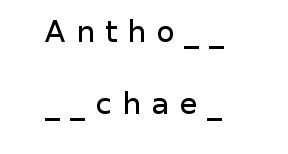
\includegraphics[width=0.25\textwidth]{wheel_of_fortune_example}
    \caption{These are two words with a handful of letters left out. It is not hard to guess the correct words, especially if told these are names. A computer, with access to a lexicon, can be far more effective at this guessing game than a human.}
    \label{fig:wheel_of_fortune_example}
\end{figure}

In our method, a partial recognition (the known letters of the ``game'') would be achieved by spotting frequently occurring character n-grams in handwritten documents. Character n-grams are simply groups of n consecutive characters, such as ``ar'' or ``ing'' (our work will focus on using bigrams and possibly trigrams); all words can be viewed as being made of a set of character n-grams. Character n-grams are useful as they occur with far greater frequency than individual words, and are more distinguishable than individual letters. With this technique, a parallel CAT system could be constructed which allows a computer and multiple humans to work in concert to transcribe a corpus. This system particularly relies on very minimalistic human input (typically selecting things).




%%%%%%%%%%%%%%%%%%%%%%%%%%%%%%%%%%%%%%%%%%%%%%%%%%%%%%%%%%%%%%%%%%%%%%%%%%%%%%%
\section{Related Work}

Segmentation is a difficult part of handwriting recognition. While line segmentation techniques are able to accurately extract lines of text and with good success extract words, letter segmentation is an open problem. In the 2013 ICDAR handwriting segmentation contest, multiple entries achieved close to 99\% line segmentation detection and accuracy, while the best word segmentation method achieved 91\% accuracy\cite{icdar_segmentation2013}.

Whole word recognition is infeasible for large vocabularies, so we would prefer to recognize individual characters. But to properly segment the letters from a handwritten word (particularly if it is written in a cursive script) is extremely challenging without the transcription. This is Sayre's paradox, where the segmentation and recognition are dependent on one another.\cite{sayres} To solve this, the state-of-the-art approaches have tried to recognize and segment simultaneously.

Hidden Markov models (HMM) were borrowed from speech recognition to accomplish this task, and worked reasonably well\cite{Marti2001}. However, HMMs have their own limitations, particularly the Markov assumption and the fact that they are most effective with windows less than the length of a letter, meaning context is often lost.

Recurrent neural networks (RNN) do not have the same limitations as HMMs, and have passed HMMs in performance\cite{Graves2009hmm}. However, they are still lacking the accuracy that is needed for a reliable automatic transcription system; the state-of-the-art results for RNNs (employing long short-term memory blocks) still may have a word error rate above 25\% when transcribing a historical corpus\cite{icdarComp2015}.



Due to the limitations of current handwriting recognition methods, we believe that a fully automated handwriting transcription is out of reach with the present of technology. We thus turn our attention to semi-automated recognition approaches, where we are still using a human to transcribe, but also some intelligent recognition technology. A semi-automated solution will outperform a fully automated system in terms of accuracy and is still far more effective than completely manual transcription. Standard CAT approaches use human feedback to correct automatic transcription in an intelligent way, such that it learns something from the corrections. An active learning approach to handwriting transcription is similar to CAT, but is not concerned about achieving human level accuracy, just better accuracy, and thus requires less human involvement~\cite{Serrano2010}. Since we wish to have a system with accuracy comparable to human performance, thus we will focus on CAT approaches.

Toselli et al\cite{Toselli2007} have explored the realm of CAT using the idea of user-verified prefixes. They use a fairly standard HMM recognition model as the backbone of their approach, and take advantage of the incremental nature of the Viterbi decoding algorithm. The recognition is done for a line of text and the user corrects the first error. The Viterbi decoding is then run again, but this time using the assumption that everything occurring before the correction is correct, and thus reusing the computation up to that point. They have also explored slight variations of the same approach that enable more fluent user input with a touchpad\cite{Toselli2008}, mouse\cite{Toselli2009}, or multimodal means\cite{Toselli2010} which speed up the transcription process by allowing more intuitive user interaction (Fig.~\ref{fig:Toselli_multimodalCAT}). Their approach relies on a language model to make corrections on a line when a supervision is made. This means this method cannot be used to effectively transcribe documents containing non-sentence writing, such as tables and lists. Serrano, et al also have pursued a similar approach, where the user corrects the $n$ words in which the recognition model had the least confidence\cite{Serrano2014}.

\begin{figure}
    \centering
    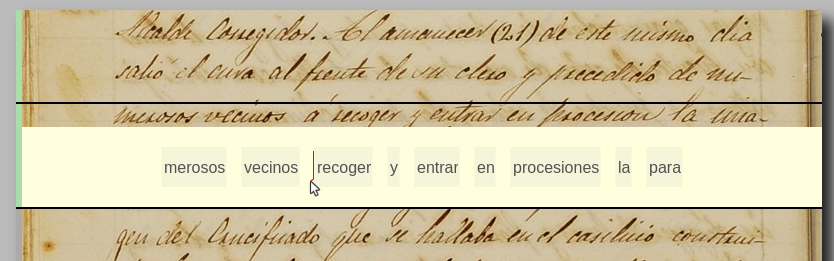
\includegraphics[width=0.95\textwidth]{Toselli_multimodalCAT}
    \caption{A screenshot of a demo of Toselli et al's multimodal CAT system. The red line is drawn by the user to indicate the need to insert a word into the automatically obtained transcription.}
    \label{fig:Toselli_multimodalCAT}
\end{figure}

While it is useful to employ an automatic handwriting recognition method as part of a CAT approach to reduce the human burden, we cannot use the same type of recognition used in most CAT systems, where there is a reliance on the predictive capacity of a language model. Some documents are not comprised of only sentences, and thus cannot be transcribed by these methods. However, many documents are structured such that a pattern can be learned to assist in transcription.

Robert Clawson\cite{Clawson2014}\footnote{You can view a short demo and explanation of his approach at \url{https://www.youtube.com/watch?v=gqdVzEPnBEw}} designed a CAT system for handwritten tabular documents, which have a clear pattern. His approach relied on simply finding matches in the document column of the current word image and assigning them the same user-specified label, as seen in Fig.~\ref{fig:ii}. This provides an accurate CAT system where the user oversees all transcription. The user oversight of matches was accomplished by showing a list of matches to the user (with an adjustable threshold for sensitivity) from which the user removed the false-positive matches. This leveraged the human user's natural ability to discriminate. However, the approach as a whole is limited as it requires frequent word repetition to be effective. While some tabular documents have this, it is not true for most other documents. Additionally, this method required a very computation preprocessing stage in which a similarity score of all words in a column with all other words in the column had to be computed.

\begin{figure}
    \centering
    \begin{subfigure}[t]{0.46\textwidth}
    		\centering
    		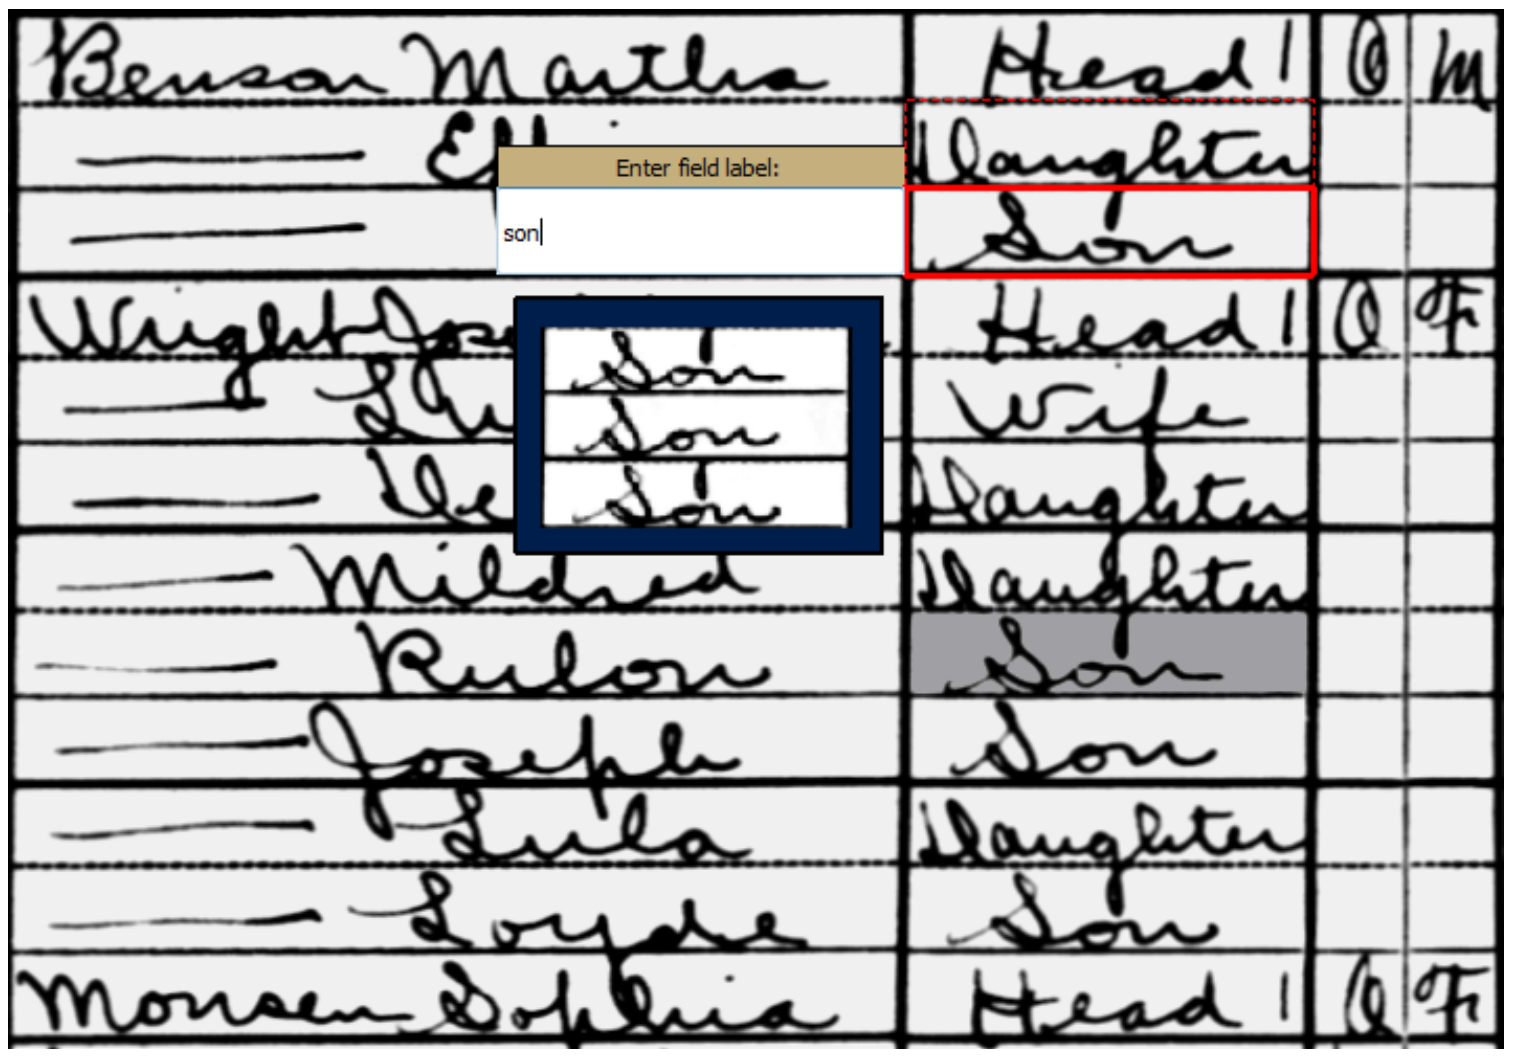
\includegraphics[width=\textwidth]{ii_ex_a}
    		\caption{A small window shows the user matching words later in the column. The user can get rid of bad matches by either clicking on them or adjusting a  threshold.}
    	\end{subfigure}
    	~
    	\begin{subfigure}[t]{0.46\textwidth}
    		\centering
    		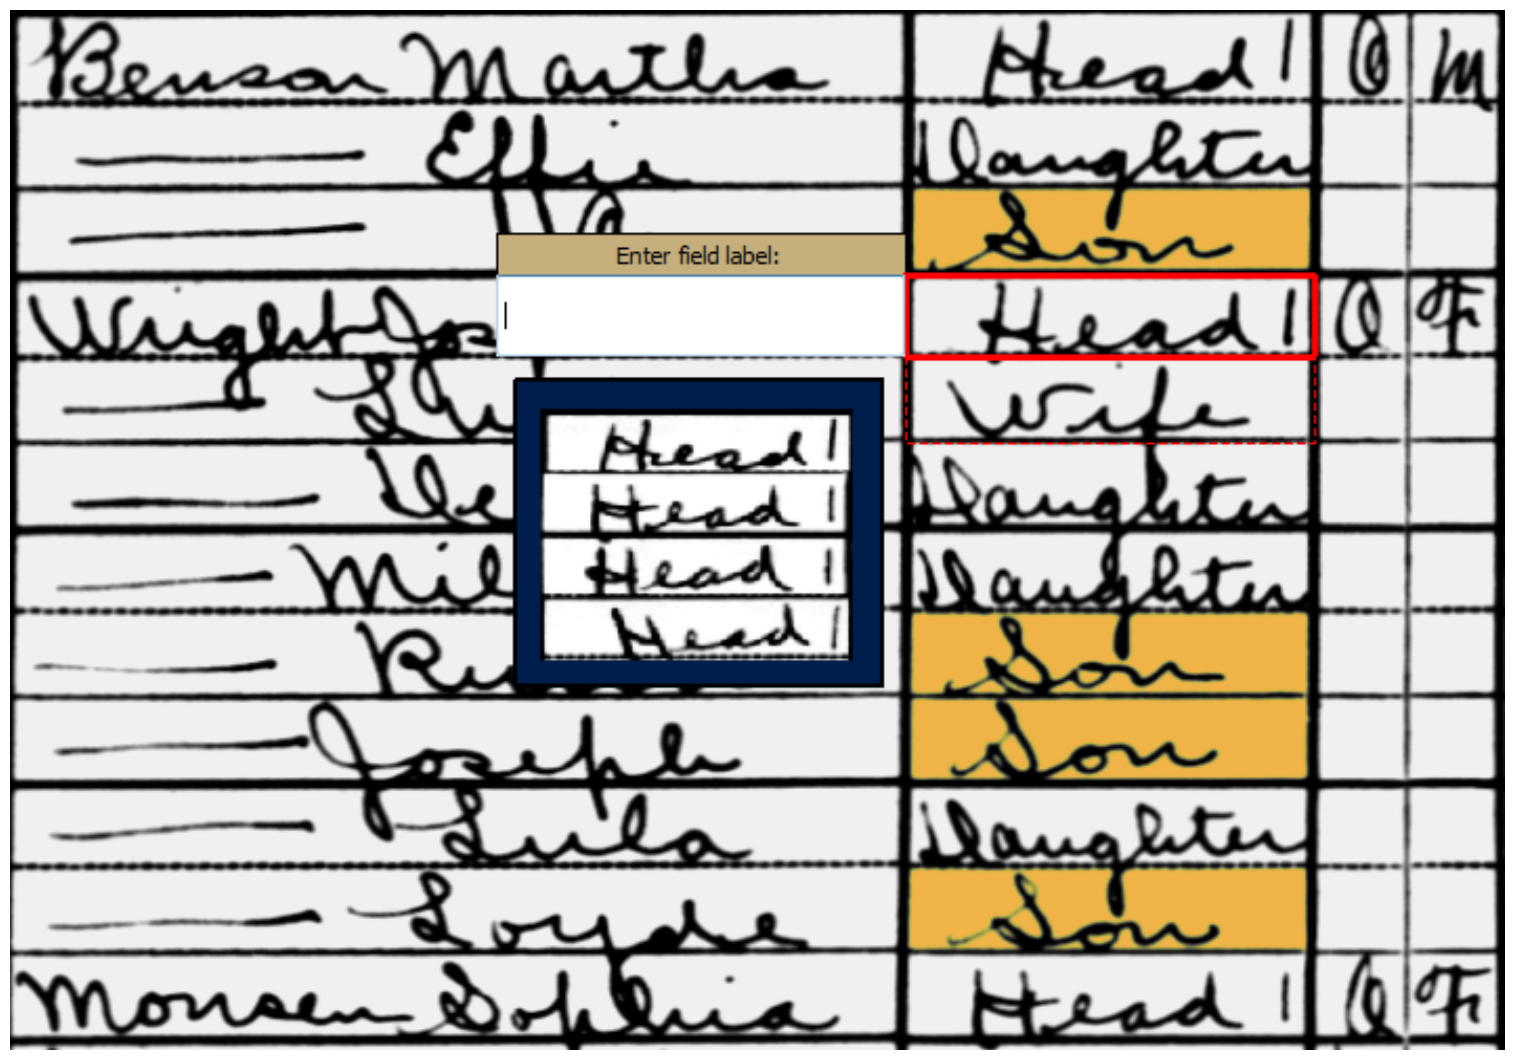
\includegraphics[width=\textwidth]{ii_ex_b}
    		\caption{The matched words are given the same label when entered.}
    	\end{subfigure}
    	\caption{Clawson's CAT system for tabular documents.}
    	\label{fig:ii}
\end{figure}

%"A Framework for Efficient Transcription of Historical Documents Using Keyword Spotting"
Zagoris et al\cite{Zagoris2015}\footnote{A demo of their system is found at \url{http://vc.ee.duth.gr/ws/}} presented a CAT system that was also based on word spotting. In their system when the user is transcribing a word image, they are presented with the results of spotting that image (sorted according to rank). The user can then confirm these spottings by clicking on them, causing them to move to a separate list. When this is done, a relevance feedback loop is activated in which submits another word spotting query of the confirmed image. These results are fused into the ranked list providing a better selection. The description of the system is unclear, but we believe the list of confirmed spottings are then labelled the same as the current word image.

Neudecker and Tzadok\cite{Neudecker2010} presented a CAT system for historical printed documents which is very similar to the CAT system we are presenting here. The system would first segment the individual characters of the documents and run an OCR engine on them. Those characters with low confidence would then be presented to a user for verification in a character session. A single character session contains all the low-confidence character images classified to a single character. An example of their system's character session for the character ``?'' is given in Fig.~\ref{fig:carpet}.  The user merely needs to select the incorrect classifications. Then in a word session, a word image is shown to the user with possible transcriptions for the word, from which they select the correct one. There are three key strengths of this system. One is that as long as the document’s characters can be segmented, it can work. The second is that it formats all user tasks as selections, rather than typing, and they are quickly completed. This creates a much more enjoyable experience for the user. The third key strength is that it is highly parallelizable for crowd-sourced transcribing. This parallelism is achieved as all character sessions are independent of one another and all word sessions are independent of one another. Our system will follow this method's pattern so it has flexibility of document types, simple user tasks and a parallelizable framework.

\begin{figure}
    \centering
    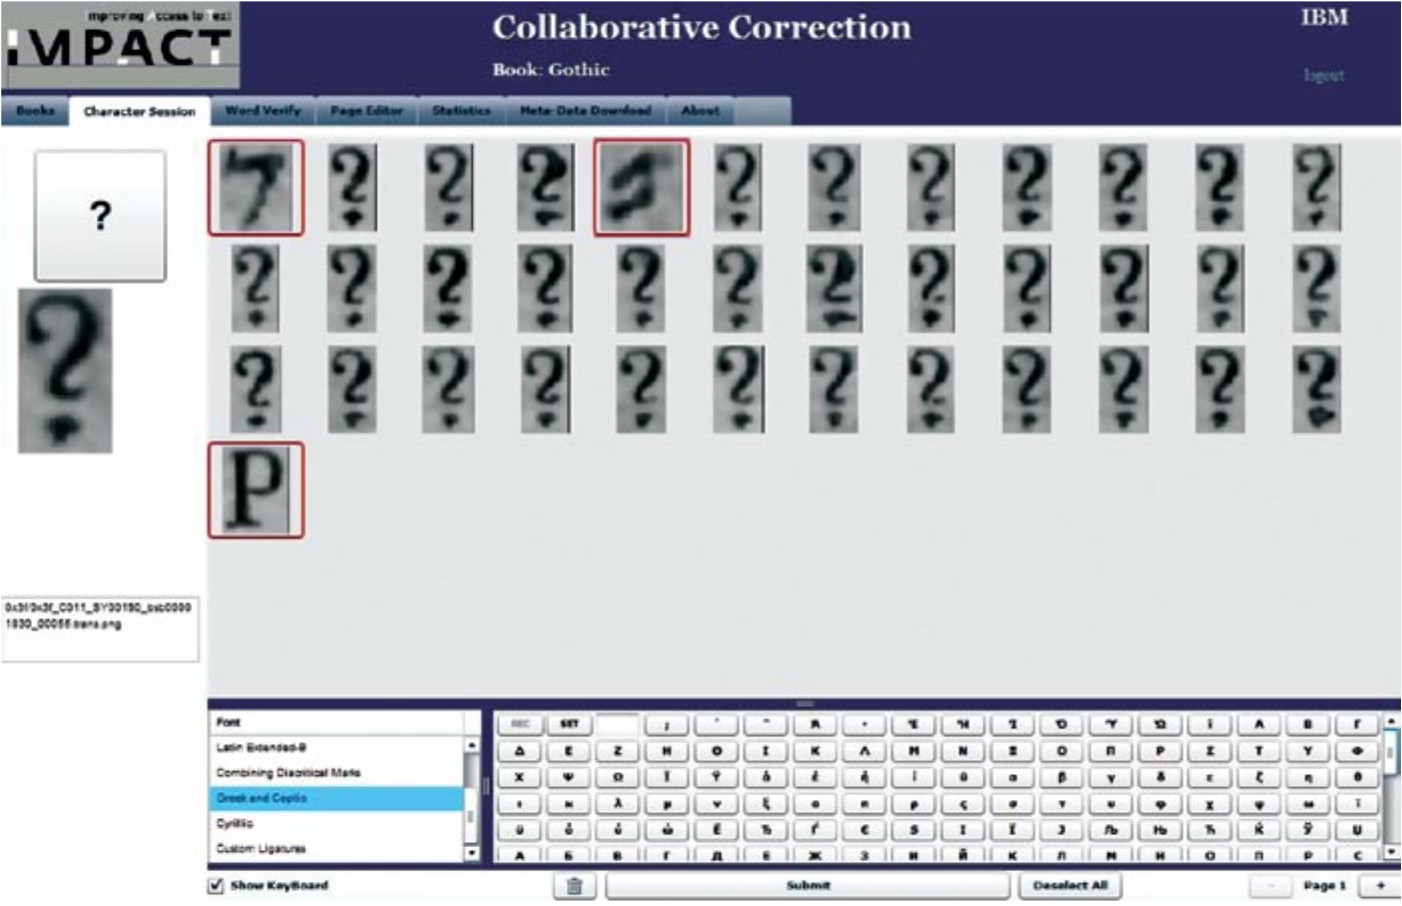
\includegraphics[width=.9\textwidth]{carpet}
    \caption{A screen shot of a character session for ``?'' from Neudecker and Tzadok's CAT system, taken directly from their report \cite{Neudecker2010}. Notice how easy it is for a user to simply click on the erroneous classifications.}
    \label{fig:carpet}
\end{figure}

Retsinas et al\cite{Retsinas2015} expanded on \cite{Neudecker2010} to reduce the amount of user input required by clustering character images together. By viewing an average of a character cluster, the user could then assign the whole cluster a character label or reject the cluster as being incoherent (the cluster contains multiple characters). Though requiring more thought from the user, this prevents the tediousness of examining all character images. Clustering could be applied to our work, it would be more difficult with handwriting, though using online learning to initialize clusters may overcome this. We, however, will not pursue it at this time.



Clawson\cite{Clawson2014} uses word spotting and user approval to transcribe, which is dependent on frequent word repetition. Neudecker, Tzadok\cite{Neudecker2010} and Retsinas et al\cite{Retsinas2015} uses OCR and user approval to transcribe, which is dependent on character segmentation, a difficult problem for handwriting.
 We will show that an alternative, a happy medium, to word spotting and OCR is character n-gram spotting, as n-grams have more frequent repetition than words do, but are large enough to spot (i.e. there is not segmentation problem). This will provide the backbone of our CAT system. As character n-gram spotting is very similar to word spotting, let us examine the literature that may be relevant to our method.

Word spotting was first proposed as an alternative to transcribing a corpus. Rather than digitizing the document text image so standard text searches can be run, the document is searched using the images themselves, either with a keyword string or a keyword image (exemplar image). There are two primary approaches to featurizing the images when word spotting: holistic features which capture information about a whole image (word) and local or sequential features\cite{Rodrıguez2008}. Holistic features have one description for an entire word image (such as a bag-of-visual-words), whereas local features have descriptor for a small portion, or window, of a word image. As local features provide much more detail and are more flexible than holistic features, they have been the most actively pursued in research.

Most of these locally directed feature approaches share the common theme of taking features from vertical slice windows (usually only one or a handful of pixels wide). They compare an exemplar using either dynamic time warping (DTW) or HMMs, relying on a prior line segmentation. The variance between the methods largely lies in the features used. Some use small square windows to allow totally segmentation-free word spotting using a sliding window\cite{Rothacker2013}.

Rodr{\i}guez et al\cite{Rodrıguez2008} proposed a simple histogram gradient feature which demonstrated improved performance when compared with (1) the popular profile and transition based features of Rath and Manmantha\cite{Rath2003}, (2) the gradient and transition focused features of Marti and Bunke\cite{Marti2001} and (3) the simple histogram features of Bunke et al\cite{Bunke2004}. They also showed that a HMM worked better than DTW, for their features. Their method was not an exemplar based approach.

Recently, Aldavert et al\cite{Aldavert2015} and Almazan et al\cite{Almazan2014} have presented superior word spotting methods which rely on heuristic descriptions. Aldavert et al use the well known bag-of-visual-words method, including recent improvements from the Computer Vision community. This is a very simple, yet effective, exemplar spotting approach. Aldavert et al use Fischer vectors, which are similar to bag-of-visual-words, with spatial pyramids in addition to a special character histogram pyramids. These are used to find a new space in training in which both strings and word images can be embedded. This allows it to perform both string and exemplar queries as well as hybrid queries which yield excellent results.

We are interested in spotting character n-grams (bi- and trigrams) rather than words. While this hasn't explicitly been done, we feel examining the performance of other methods on short words (2 to 3 letters) is instructive. For Rothacker et al's\cite{Rothacker2013} segmentation free HMM based method, they report $\sim$46\% and $\sim$55\% mean Average Precision (mAP) for two and three lettered words respectively, a drop by $\sim$15\% and $\sim$6\% from the mAP for all words they tested (61\%). Fischer et al\cite{Fischer2012} report $\sim$70\% and $\sim$83\% mAP for two and three lettered words, compared to {\textgreater}90\% mAP for words of length 5 or longer, for their line segmentation dependent, character HMM based method. While neither of these numbers are very promising, Almazan et al\cite{Almazan2012} observe that sliding window approaches can frequently find false positives of short words inside other words (e.g.~finding the word ``the'' inside the word ``weather''). As this is precisely what we want to happen in n-gram spotting (that is, we \textit{want} to find groups of letters in the middle of words), we expect we should have more success spotting character n-grams than other methods in spotting short words. However, part of the poor accuracy in spotting short words is the fact that there is less information with which to discriminate; this is an obstacle we still must overcome.


%%%%%%%%%%%%%%%%%%%%%%%%%%%%%%%%%%%%%%%%%%%%%%%%%%%%%%%%%%%%%%%%%%%%%%%%%%%%%%%
\section{Thesis Statement}


We will construct a computer assisted transcription system for handwritten documents which will partially transcribe words by completing the easier task of spotting character n-grams which occur densely throughout the corpus. These n-grams accumulate partial transcriptions that permit constrained lexicon look-ups from which users can select the correct transcription. 

%%%%%%%%%%%%%%%%%%%%%%%%%%%%%%%%%%%%%%%%%%%%%%%%%%%%%%%%%%%%%%%%%%%%%%%%%%%%%%%
\section{Project Description}

We will develop a character n-gram spotter, experimenting with modifying existing methods.
% as well as trying ones based on object detection strategies from computer vision.
This performance will be empirically measured. Using the results of the performance of the n-gram spotting, we will evaluate the size of lexicon for which our approach will be feasible.

We then will implement a demonstrative CAT tool using the flexibility of n-gram spotting. This will largely be a proof-of-concept work to show how one might use character n-gram spotting. We anticipate its performance to be good, but it may be difficult to compare to similar tools as ours will be strongest in an application that is slightly different from how most others have been tested.


\subsection{Spotting}
We require a spotting method which can learn incrementally. Image exemplar spotting approaches are an easy way of doing this as new examples can simply become new queries. However, other trained methods may be able to be updated. There are some spotting methods which are able to do both image and string based queries\cite{Almazan2014} which would be useful for leveraging both offline training and new exemplars.

Given our specific need in spotting character n-grams, we will likely have to adapt the current word spotting technology to get the performance we need. This will be a preliminary task that will provide the backbone for our CAT system.

\subsection{Preprocessing}
All documents will be preprocessed to reduce noise, deskew the image, segment lines, have the text lines deslanted and have the words segmented (if needed by the spotting method). Word segmentation will likely have errors, but these can be corrected by users.

\subsection{Lexicon}
Lexicon look-ups with wildcards is a well studied problem. An approach which would be well suited to our needs is n-gram indexing, in which each n-gram has all words which contain it indexed to it. Then a search is simply an intersection of all the indexes for the n-grams in the query.

\subsection{Tool}
The system is designed to leverage the flexibility of character n-gram spotting to create partial transcriptions. This flexibility largely comes from it's parallelizable nature; individual spotting tasks, and transcription tasks, are not dependant on one another. This allows an interactive design with multiple asynchronous users. Additionally, we can exploit user feedback to improve spotting.

We will begin by training our spotting method so that it can spot n-grams in most types of handwriting with a reasonable accuracy. This will be used to begin spotting the documents. Depending on this character n-gram spotter's performance, a training step may need to precede the main execution, allowing the spotting method to gather context/author specific n-gram exemplars. 

The system is broken into tasks, some of which are completed by the users, some of which are completed by a server doing the computation/spotting. By including a task manager which distributes tasks, we can allow for multiple users to be working on the same set of documents simultaneously. See Fig.~\ref{fig:system_diagram} for a brief outline of the work-flow. The tasks comprising the work done by the computation server and the user will be the following subsections.

This method is unique as the different user's progress will help produce more tasks, making the effort very cooperative. This happens as each completed n-gram verification task will provide partial transcriptions for words in the corpus. This allows more possible complete word transcriptions to be found. Each spotting and full word transcription that is done provides more n-gram image examples to the system from which it can improve spotting, creating more tasks for the server and then other users. This incremental learning from new n-gram example images can be done in two ways: using them as new image exemplars for queries directly or attempt to learn features from them to improve following queries. Additionally, we can use them as a refining tool to prune images returned by previous spotting tasks (that haven't been user-reviewed yet). This acts similarly to the relevance feedback of Zagoris et al\cite{Zagoris2015}.

\iffalse
[Active Learning.TODO]
Motivations:
What do we want?
-Accurate transcriptions.
-Fast transcriptions.
What do users want?
-To feel they are important/making a difference.
-Not be frustrated. Flow.
-Sense of accomplishment

What can we learn? (globally and locally adjusted to particular corpi/documents)
-learn threshold for returning positive ngram spots (we don't want users to have to discard too many false positives)
-learn threshold for showing ngrams vs. assuming they are correct (i.e. confidence in ngram spotting)
-learn threshold for picking transcription (score from spotting hypothesis word) (i.e. confidence in word spotting)
-learn which query to use next
	is reusing spotted ngrams as queries or extracting new ngram queries from words better?
	is it better to focus on most common ngrams, or to spot broadly?
-learn reliability/speed of particular users (so we can give them high priority or difficult tasks)
-learn user's state-of-mind
	are they frustrated with the tasks they're doing? (or, how likely are they to quit?)
\fi	




This prototype system will be developed as an in-browser app, thus making it immediately cross-compatible with all devices with a modern browser. A Node.js server will be created to communicate with the clients and the C++ program which will be responsible for performing the actual word spotting.

\begin{figure}
    \centering
    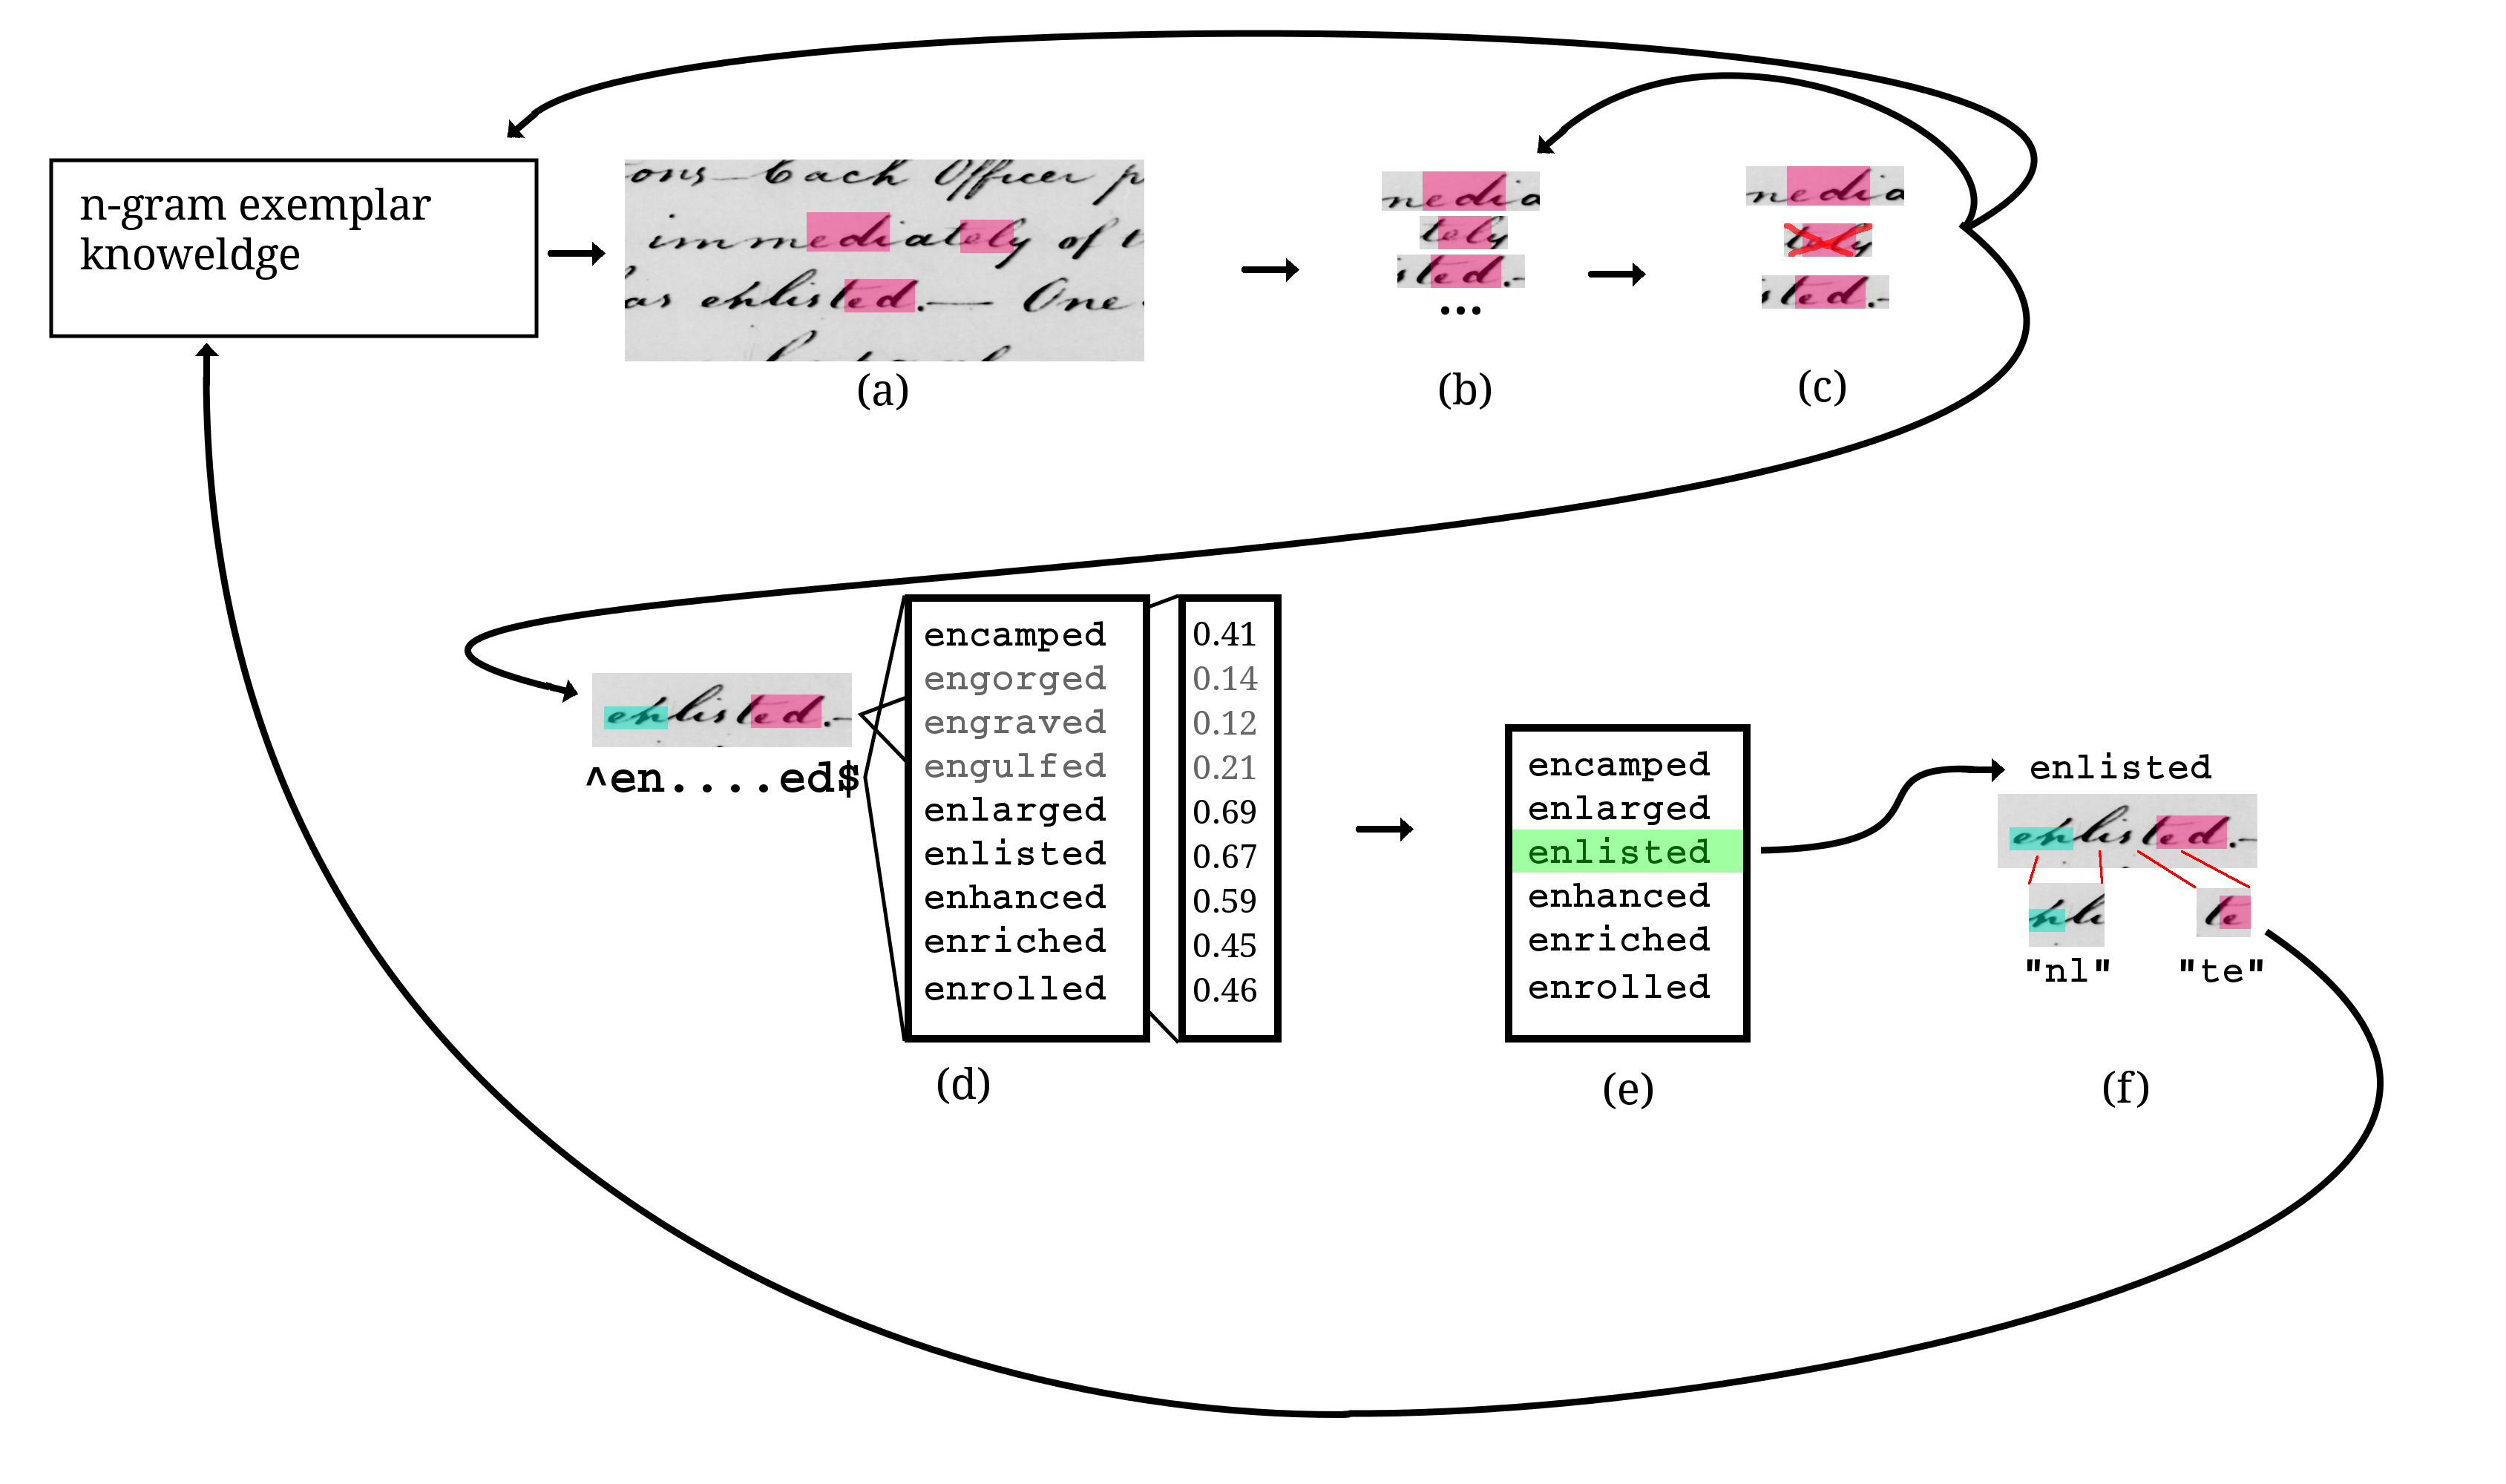
\includegraphics[width=.95\textwidth]{flow6}
    \caption{The work-flow of the proposed CAT system. (a) Server character n-gram spotting task. (b) Server n-gram verification distribution. Pools results from the previous task and distributes them to users as they become available. (c) User n-gram verification task. Passes it's results both forward (towards transcription) and backward (incremental learning and relevance feedback). (d) Server lexicon look-up and scoring task. A regular expression is generated from all currently spotted n-grams (``en'' and ``ed'' in this example). The regular expression generates a list of possible transcriptions and a word spotting/recognition algorithm scores each of these on the image. If the number of words above some threshold is small (black words), they are passed to a user. (e) User transcription selection task. (f) Extracting new n-gram exemplars which are used for incremental learning.}
    \label{fig:system_diagram}
\end{figure}


\subsubsection{Computation Server Tasks}

{\setlength{\parindent}{0cm}
\textbf{Character n-gram spotting}

\begin{addmargin}[3em]{3em}
Select the most promising n-gram exemplar to spot; this is based on the frequency of n-grams and whether we have new information for an n-gram from document/author specific examples extracted from transcribed text. Spot that n-gram in the documents. The spotting scores will be thresholded at a certain level for discarding negative. Another threshold will accept spottings as positive matches. The remaining results (medium confidence) will be reserved as unsure and incrementally distributed to users for n-gram verification.
\\[.5cm]
\end{addmargin}

\textbf{Character n-gram verification distribution}

\begin{addmargin}[3em]{3em}
This is closely related to the above task. It, however, additionally receives feedback from the users' n-gram verification task. As spotted images are returned labeled as true-positive or false-positive, we can refine the list of spottings waiting to be verified by users. Based on their similarity to an accepted or rejected image, spottings waiting for review will have their confidence adjusted. Additionally, the thresholds used for that particular spotting may be adjusted. This will cause some spottings (yet to be reviewed) to now be above or below the threshold(s) allowing the system to automatically decide whether they are a true- or false-positive, thereby pruning the list (or possibly expanding the list, if the cut-off threshold was too high).


\-\hspace{1cm} As users finish tasks, this distributes new tasks based on whether a particular n-gram has pending feedback and whether that feedback will be useful. Suppose the system just spotted the bigram ``an'' and has three users completing the first n-gram verification tasks. It would be more valuable to assign some other task (not ``an'' verification) to a ready user; if we wait until the users doing the ``an'' tasks are finished, their results will prune the list of spottings waiting to be verified, thus reducing possibly redundant work.
\\[.5cm]
\end{addmargin}

\textbf{Lexicon look-up and scoring}

\begin{addmargin}[3em]{3em}
When a word has roughly 20\% of its area labelled by n-grams, we create a regular expression representing what we know. This is based on the position of the n-grams in the word, using flexible wildcards to specify possible unrecognized characters and their position which we estimate from the image (the ``Wheel of Fortune'' game). If the list of returned words is small (perhaps less than 40), we performing a scoring of them by running a word spotting or handwriting recognition algorithm on the word image scoring for each of the possible transcriptions. We can then discard any possible transcriptions scoring below a threshold. This threshold can be adaptive to the distribution of the particular set of scores. If few words are above the threshold (10 or less) we pass this to the user for the transcription selection task (where the user selects the correct transcription from the returned words). If only one word is returned, either from the initial look-up or from the score pruning, we can transcribe the word without human intervention.
\\[.5cm]
\end{addmargin}

\textbf{Incremental learning}

\begin{addmargin}[3em]{3em}
After the user has confirmed a transcription for a word image, we can then extract new character n-gram exemplars from the image, using the spatial information we have from the n-grams spotted in the image. Additionally, confirmed n-gram images we already spotted can be new exemplars. Both of these new exemplars can be author specific which will greatly improve spotting for pages with the same author. How the exemplar is used will depend on the final spotting algorithm selected; it may either be used directly as a query, to modify a query, or as means to learn new character models.


\-\hspace{1cm} Additionally, based on n-gram verification and transcription tasks, we can adjust the following parameters to better fit the documents being transcribed: the confidence threshold for automatically accepting or rejecting n-gram spottings and the threshold for automatically accepting a hypothesis transcription based on the its word spotting score.
\\[.5cm]
\end{addmargin}
}


\subsubsection{User Tasks}





{\setlength{\parindent}{0cm}
\textbf{Character n-gram verification} (Fig.~\ref{fig:userTask_spot})

\begin{addmargin}[3em]{3em}
The user is shown segments of the image where the spotted n-grams are highlighted. The user selects any false-positives. The assumption is that most should be correct, thus making it easy to pick out those not belonging to the set.
\\[.5cm]
\end{addmargin}

\begin{figure}
    \centering
    
\includegraphics[width=.4\textwidth]{userTask_spot}
    \caption{A mock-up of what the user might see when verifying character n-gram spotting. The highlighted images are from the server spotting a particular n-gram. The red-boxed image has been selected by the user as it is a false-positive.}
    \label{fig:userTask_spot}
\end{figure}

\textbf{Select correct transcription} (Fig.~\ref{fig:userTask_trans})

\begin{addmargin}[3em]{3em}
The word being transcribed is highlighted and is presented to the user with the list of possible transcriptions (ordered by the likelihood of the possible transcriptions and the score generated from word spotting the image). The user either selects the correct transcription, or corrects the search by doing one or more of the following:
\begin{itemize}
    \item Splitting the image into two words.
    \item Indicating the image is splicing a word (and which side).
    \item Indicating if any of the n-gram labels are wrong (in case of earlier human error).
    \item Manually entering the transcription.
\end{itemize}

\end{addmargin}
}

\begin{figure}
    \centering
    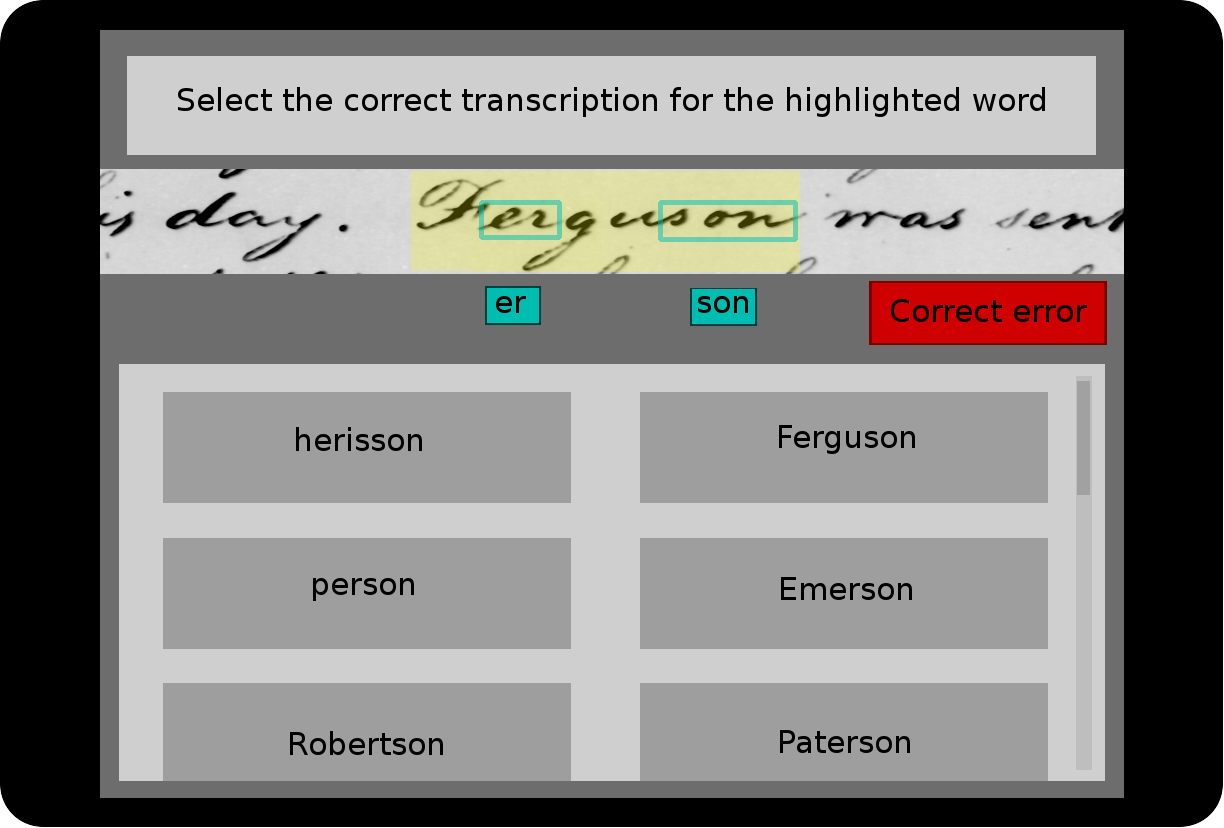
\includegraphics[width=.6\textwidth]{userTask_trans}
    \caption{A mock-up of what the user might see when selecting a correct transcription. The transcription possibilities are returned from the server's lexicon look-up.}
    \label{fig:userTask_trans}
\end{figure}


\subsection{An Example}
To solidify our description of our transcription system, let us examine a very specific example of how our system would transcribe a word, ``there,'' in a corpus. The word ``there'' occurs 15 times in the George Washington (GW) dataset\cite{GW}. The bigram ``\texttt{th}'' being the most common in the English language would be the first one spotted. We are presuming that our spotting method has 49\% recall. The system would spot roughly 7 of the ``th''s in the ``there''s of the corpus, along with other ``th''s in other words and false positives. The ``th''s are presented to a user to clean out the false positives. Let us assume this is done perfectly and there are no false positives remaining. Having ``th'' spotted at the beginning of a word ``there'' would allow us to create the regular expression \texttt{{\textasciicircum}th....?\$} (the extra \texttt{.?} to represent uncertainty about the number of characters present in the word) for each of these instances, which will return 60 different transcriptions from a 32,000 word lexicon. These are scored and thresholded usign a word spotting/recognition algorithm reducing the list to 30 possible transcriptions. This is too many to present to a user so we continue spotting. The fourth bigram that would be spotted is ``\texttt{er}.'' Let us say the ``er'' is spotted in 4 of the ``there''s we've spotted ``th''s in, allowing us to create the regular expression \texttt{{\textasciicircum}ther..?\$} for them. This returns only the words ``there'' and ``there's'' (let's assume the lexicon is stripped of non-word characters), which being very similar are not scored differently enough by our word spotting/recognition to automatically prune. We can transcribe these 4 words by simply presenting the two options to the user and having him/her select the correct transcription. We can use the ``th''s and ``er''s we did spot correctly for creating new queries for subsequent spotting iterations, which may catch the ``th''s or ``er''s we missed previously. Additionally, we can extract  ``re'' examples from the ``there''s we have transcribed, by estimating their location, based on the location of the ``er''s we spotted.

TODO figure for above

%Let's examine another example, the word ``enlisted'' which occurs three times (see Fig.~\ref{fig:system_diagram}). 

\subsection{Preliminary Work}

\subsubsection{Subword Spotting}
We have begun testing state-of-the-art word spotting methods under the application of spotting bigrams and trigrams within words. Our best results so far have been Almazan et al\cite{Almazan2014}, which achieved 64\% mAP spotting bigrams and 72\% mAP spotting trigrams in the George Washington dataset.

\subsubsection{System Simulation}
In an attempt to justify our method, we created a simulation to discover how many tasks would need to be completed by users if we were transcribing a given corpus. This simulation takes a number of parameters: a recall rate for an imaginary subword spotting method, a rough confidence level for counting the number of unrecognized characters in a word, and a cut off for the number of possible transcriptions a word must be narrowed to before counting the word as transcribed. The real system would send a transcription selection task to the user, but we don't feel the need to simulate this. We ignore the precision of our imaginary spotting method as all spotting is verified by the user, so given no user error, it will have 100\% precision. However, the recall of the system will be balanced with how much work the user has to do in these tasks; this is important in our selection/development of a subword spotting method, but not to our simulation.

%TODO lookup if 10 is a good number
We have held the possible transcription cut-off at 10, as we feel that is a reasonable number for a user to deal with. We used a recall rate of 49\%, as this should correspond to an acceptably high accuracy rate give 64\% mAP. The results presented here are from a simulated transcription of the 20-page George Washington dataset. We used a 32,000 word lexicon and spotted only the 100 most frequent bigrams.

%To solidify our description of our transcription system, let us examine a very specific example of how our system would transcribe a word, ``there,'' in the corpus and how the simulation represents this. The word ``there'' occurs 15 times in the GW corpus. The bigram ``\texttt{th}'' being the most common in the English language would be the first one spotted. We are presuming that our spotting method has 49\% recall. The system would spot roughly 7 of the ``th''s in the ``there''s of the corpus, along with other ``th''s in other words and false positives. We simulate this at each ``th'' by having a 49\% change of ``spotting'' the ``th''. In the real system, the spotted ``th''s are presented to a user to clean out the false positives. In our simulation, we assume this is done and there are no false positives. Having ``th'' spotted at the beginning of a word ``there'' would allow us to create the regular expression \texttt{{\textasciicircum}th....?\$} (the extra \texttt{.?} to represent uncertainty about the number of characters present in the word) for each of these instances, which will return 60 different transcriptions from the lexicon. This is too many to present to a user so we continue spotting. The fourth bigram that would be spotted is ``\texttt{er}.'' Let us say the ``er'' is spotted in 4 of the ``there''s we've spotted ``th''s in, allowing us to create the regular expression \texttt{{\textasciicircum}ther..?\$} for them. This returns only the words ``there'' and ``there's'' (let's assume the lexicon is striped of non-word characters) and so we can transcribe these 4 words by simply presenting the two options to the user and having him/her select the correct transcription. We can use the ``th''s and ``er''s we did spot correctly for create new queries for subsequent spotting iterations, which may catch the ``th''s or ``er''s we missed previously. Additionally, we can extract  ``re'' examples from the ``there''s we have transcribed, by estimating their location, based on the location of the ``er''s we spotted.

In Fig.~\ref{fig:fullSim} we can see the progress of the simulation through the series of tasks. As might be expected, the rate of transcription begins to drop off as most of the words are transcribed. It will be necessary to stop transcription through n-gram completion at some point and do manual transcription for the remaining words. However, this demonstrates the feasibility of our method. Within 250 spottings, 75\% of the corpus is transcribed (including out-of-vocabulary words).

\begin{figure}
    \centering
    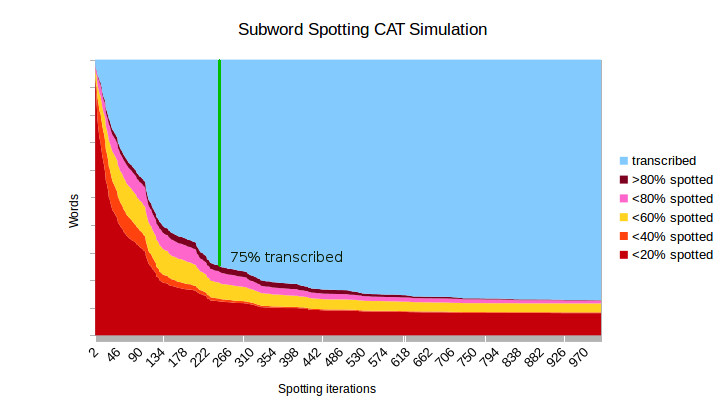
\includegraphics[width=1.0\textwidth]{simulationGraph_line}
    \caption{A simulation run with medium confidence on unspotted character count prediction. The chart is drawn so one can observe the progress of spotting as well as transcription, each category indicating the portion of words which have the given percent of their characters recognized by spottings (or indicating the portion of words transcribed). One will note that a large number of words never have more than 20\% of their characters spotted. This is due to two reasons: we are only using the 100 most frequent bigrams, and many of words in the corpus are numbers, which we are not spotting or transcribing in this simulation. The group of words which are between 40\% and 60\% spotted which are never transcribed are either out-of-vocabulary as well or are simply diabolic cases which have too many possible transcriptions given the limited number of bigrams we can spot. An example of this diabolic case is the words ``suffice.'' The only bigrams we spot that are present in the word are ``ic'' and ``ce'' and the number of seven letter words ending in ``ice'' is 17 for our dictionary, thus this word would never be ``transcribed'' in the simulation.}
    \label{fig:fullSim}
\end{figure}

A parameter our simulation is very sensitive to, which we assume the actual system will be sensitive to as well, is the confidence in predicting the number of characters in a word which are not spotted. If given a low confidence, such that the simulation searched more possible transcriptions, the simulation saturated transcription at around 66\% transcribed at 350 iterations (spottings) and failed to move past 71\% by 1000 iterations. If given perfect knowledge of how many characters are present, but not spotted, the system achieves 66\% after only 127 iterations and does not saturate until about 86\% has been transcribed. From further analysis, we see that it is caused by many words being transcribed as much as they can be (given the limited n-gram set), but still not returning a possible transcription count below the threshold of 10. If the prediction of the number of unspotted characters proves to be difficult, a loosening of this threshold as the corpus is transcribed may be required.



%%%%%%%%%%%%%%%%%%%%%%%%%%%%%%%%%%%%%%%%%%%%%%%%%%%%%%%%%%%%%%%%%%%%%%%%%%%%%%%
\section{Validation}
The n-gram spotting methods will be empirically tested using well known datasets (George Washington\cite{GW} and IAM\cite{IAM}) as well as a dataset closer to the domain of our expected application of the transcription method.

\subsection{User Study}

Our CAT system must be validated with a user study as it's goal is to be a more effective crowdsourcing method for transcription. It is not purely intended to be faster (indeed, it may not be faster than other computer assisted transcription methods), but more modular, allowing for work to be broken up into smaller pieces, and more enjoyable to use. It clearly achieves modularity in design, but we want to see how fast it is and get user feedback to see if it is something people would enjoy using.

Most other computer assisted transcription methods rely on a more fully automated transcription upfront and report performance measures in terms of word error rate or effort reduction, which are measures of how many words the user had to correct. While our users will primarily be doing corrections as well, they will very different types of corrections, that is, merely rejecting bad n-gram spottings instead of typing new transcriptions. Thus it would be difficult to compare these other methods to our proposed method using the previous authors' metrics, though they still may prove to be useful.

We propose doing a user study which would involve having a volunteer\footnote{Recruiting volunteers can be aided by using Robert Clawson's volunteer testers list as a starting place. The rest will be gathered via on-campus flyers and personal connections.} use the system for about 5-10 minutes on their own device at their own convenience. This is probably the easiest way to get a large number of participants and a varying degree of experience transcribing documents among the volunteers. To encourage use on more platforms, so that we get a broader survey, the study will encourage users to use tablets and phones.
We will track what device they use, how many tasks they complete, how long it takes them to complete tasks, and errors they make, in addition to having the volunteers complete a short survey about their experience.

Given the flexibility of the system, we would like to test it on two different document types: a regular written text like the George Washington\cite{GW} or the Jennie Leavitt Smith\cite{Smith} dataset, and a structured dataset such as census or marriage records. This will provide us with some comparison to Toselli's CAT approaches (which work on corpora similar to the George Washington dataset) and Clawson's CAT (which works on tabular documents).

It will be difficult to get a synchronized group of testers to explore the parallel nature of our method. Instead, we will complete a number of spotting verification tasks, and possibly transcription selection tasks, prior to having the users begin. These can then be fed to the system during a user test to simulate having other users on the system, although it may suffice to simply feed them the the system prior to the user interacting.

We will be able to measure success if the users report that system being enjoyable to use and the system works accurately (near manual transcription's accuracy). Additionally, it would be a failure if the system proves slower than manual transcription.


%%%%%%%%%%%%%%%%%%%%%%%%%%%%%%%%%%%%%%%%%%%%%%%%%%%%%%%%%%%%%%%%%%%%%%%%%%%%%%%
\section{Thesis Schedule}
\begin{table}[h]
\centering
\begin{tabular}{ll}
Finalization of spotting method          & 1 March 2016 \\
Complete implementation of UI/backend    & 15 May 2016    \\
Complete user tests                      & 1 July 2016   \\
Complete revisions                       & 1 August 2016      \\
Complete additional user tests           & 15 September 2016     \\
Thesis written (all but final revisions) & 1 December 2016     \\
Thesis defended                          & 30 January 2017    
\end{tabular}
\end{table}


%%%%%%%%%%%%%%%%%%%%%%%%%%%%%%%%%%%%%%%%%%%%%%%%%%%%%%%%%%%%%%%%%%%%%%%%%%%%%%%
% Change these to reflect the bibliography style and bibtex database file you want to use
\bibliographystyle{plainnat}
\bibliography{bib}

\end{document}
